\documentclass[a4paper,12pt]{report}
\usepackage[top=1cm, left=1cm, right=1cm, bottom=1.5cm]{geometry}
\usepackage[T1]{fontenc}
\usepackage{hyperref,graphicx,amsmath,pdfpages,float}
\begin{document}
\begin{center}
    \large \textbf{CHE613A: The Structure \& Rheology Of Complex Fluids\\(Assignment 2)}
\end{center}

\begin{flushright}
    Keerthi Vasan M\\Roll No.: 21102023\\keerthi21@iitk.ac.in\\ \today
\end{flushright}
\vspace{-5mm}
\rule{\textwidth}{0.5 pt}
\noindent
\textbf{Question no.: 01} By using the data for variation of viscosity with respect to temperature obtain activation energy for flow in kJ/mol for three different liquids. Furthermore, mention latent heat of vaporization in kJ/mol (at the mean of above considered temperatures) and compare the same. Please mention the reference(s).\\[2mm]
\textbf{Answer:} Reference: Viscosities of Simple Liquids - Temperature Variation. (2021, March 7). Retrieved August 19, 2021, from https://chem.libretexts.org/@go/page/96239\\As stated on the literature, variation of viscosity with temperature for water, ethanol, and diethyl ether are as follows:
    

\begin{table}[H]
\centering

\begin{tabular}{|c|c|c|c|c|c|}
\hline
\multicolumn{2}{|c|}{\textbf{Water}} & \multicolumn{2}{c|}{\textbf{Ethanol}} & \multicolumn{2}{c|}{\textbf{Diethyl ether}} \\ \hline
\textbf{Temperature ($^{\circ}$C})  & \textbf{$\eta$ (cP)}  & \textbf{Temperature ($^{\circ}$C)}   & \textbf{$\eta$ (cP)}  & \textbf{Temperature ($^{\circ}$C)}      & \textbf{$\eta$ (cP)}     \\ \hline
20 & 1.002  & 0  & 1.773 & -20 & 0.362  \\ \hline
30 & 0.7975 & 10 & 1.466 & 0   & 0.2842 \\ \hline
40 & 0.6529 & 20 & 1.200 & 20  & 0.2332 \\ \hline
50 & 0.5468 & 30 & 1.003 & 25  & 0.222  \\ \hline
60 & 0.4665 & 40 & 0.834 & 40  & 0.197  \\ \hline
70 & 0.4042 & 50 & 0.702 & 60  & 0.166  \\ \hline
80 & 0.3547 & 60 & 0.592 & 80  & 0.140  \\ \hline
90 & 0.3147 & 70 & 0.504 & 100 & 0.118  \\ \hline
\end{tabular}%
\end{table}

\noindent One of the simplest model to explain the relationship between viscosity and temperature assumes that viscosity ($\eta$) depends on the temperature ($T$) as follows:
$\eta = A \exp \left(\dfrac{E_a}{RT} \right) \label{3}$ Here $A$ is a constant (also known as pre-exponential factor), $T$ is the absolute temperature (in K), $R$ is the universal gas constant (J/mol K) and $E_a$ is the activation energy (J/mol). Upon linearization, above equation reduces to $\ln \eta = \ln A + \left( \dfrac{E_a}{R} \right) \dfrac{1}{T} \label{4}
$. Using the above mentioned viscosity-temperature data table and the linearized model equation, we can obtain the fluid flow's activation energy from the slope of the plot. 
\begin{center}
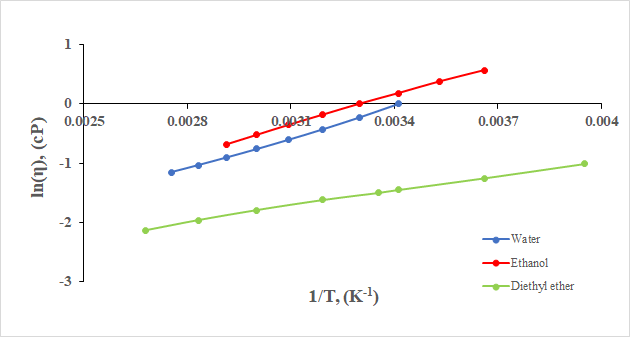
\includegraphics{plot.png}    
\end{center}
From the above plot following results were calculated, and shown below. It can be seen that the activation energy should be less than the heat of vaporization by a factor of 0.4. In other words, upper bound value for bond activation energy of a fluid is the latent heat of vaporization of that fluid.
\begin{table}[H]
\centering
\resizebox{\textwidth}{!}{%
\begin{tabular}{|c|c|c|c|}
\hline
\textbf{Fluid} &
  \textbf{\begin{tabular}[c]{@{}c@{}}Slope $\left(\dfrac{E_a}{R} \right)$\\ (K)\end{tabular}} &
  \textbf{\begin{tabular}[c]{@{}c@{}}Activation energy $(E_a)$\\ (kJ/mol)\end{tabular}} &
  \textbf{\begin{tabular}[c]{@{}c@{}}Latent heat of vaporization $\left(\approx \dfrac{E_a}{0.4} \right)$\\ (kJ/mol)\end{tabular}} \\ \hline
Water         & 1753.224 & 14.576 & 36.440 \\ \hline
Ethanol       & 1690.136 & 14.051 & 35.129 \\ \hline
Diethyl ether & 866.1372 & 7.201  & 18.002 \\ \hline
\end{tabular}%
}
\end{table}

\noindent
\textbf{Question no.: 02} If ordinate (vertical axis) is $f(t)$ and abscissa (horizontal axis) is $t$, represent following functional forms in terms of unit step functions and obtain Laplace transform of the same. Please note that: $L(u(t -a)f(t -a))=e^{-as}F(s)$ (You may have to use other Laplace transforms to including that of mentioned on the last page to obtain the results). You may find following website useful to understand the topic:
http://www.intmath.com/laplace-transformation/intro.php\\[2mm]
\textbf{Answer:} \\[1 cm]
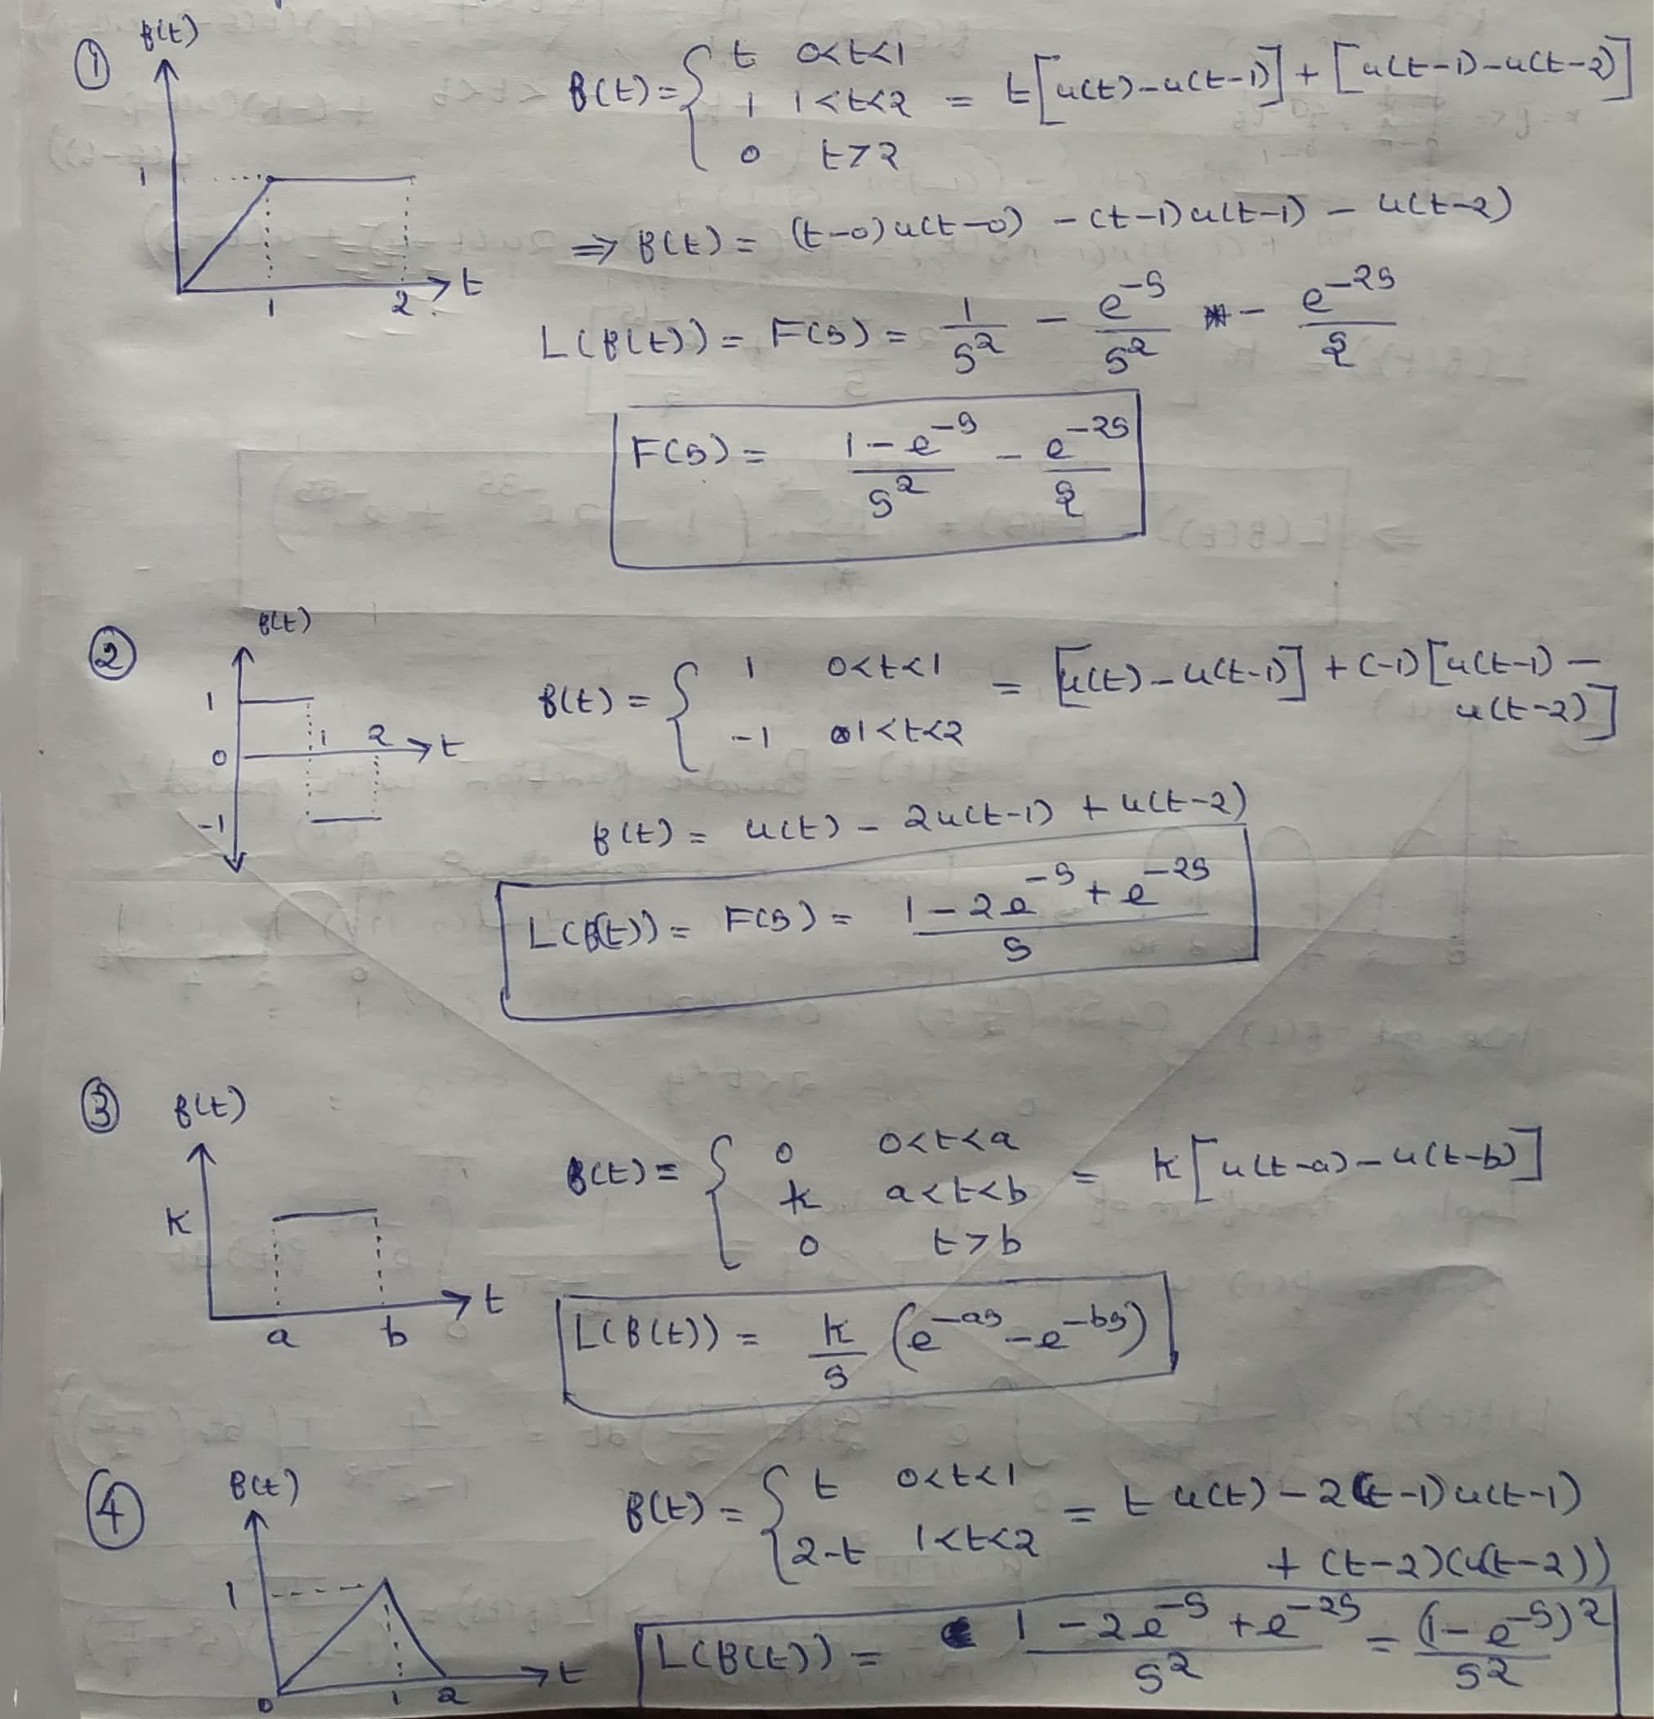
\includegraphics[scale=0.3]{CF_Assignment02_1.jpg}
%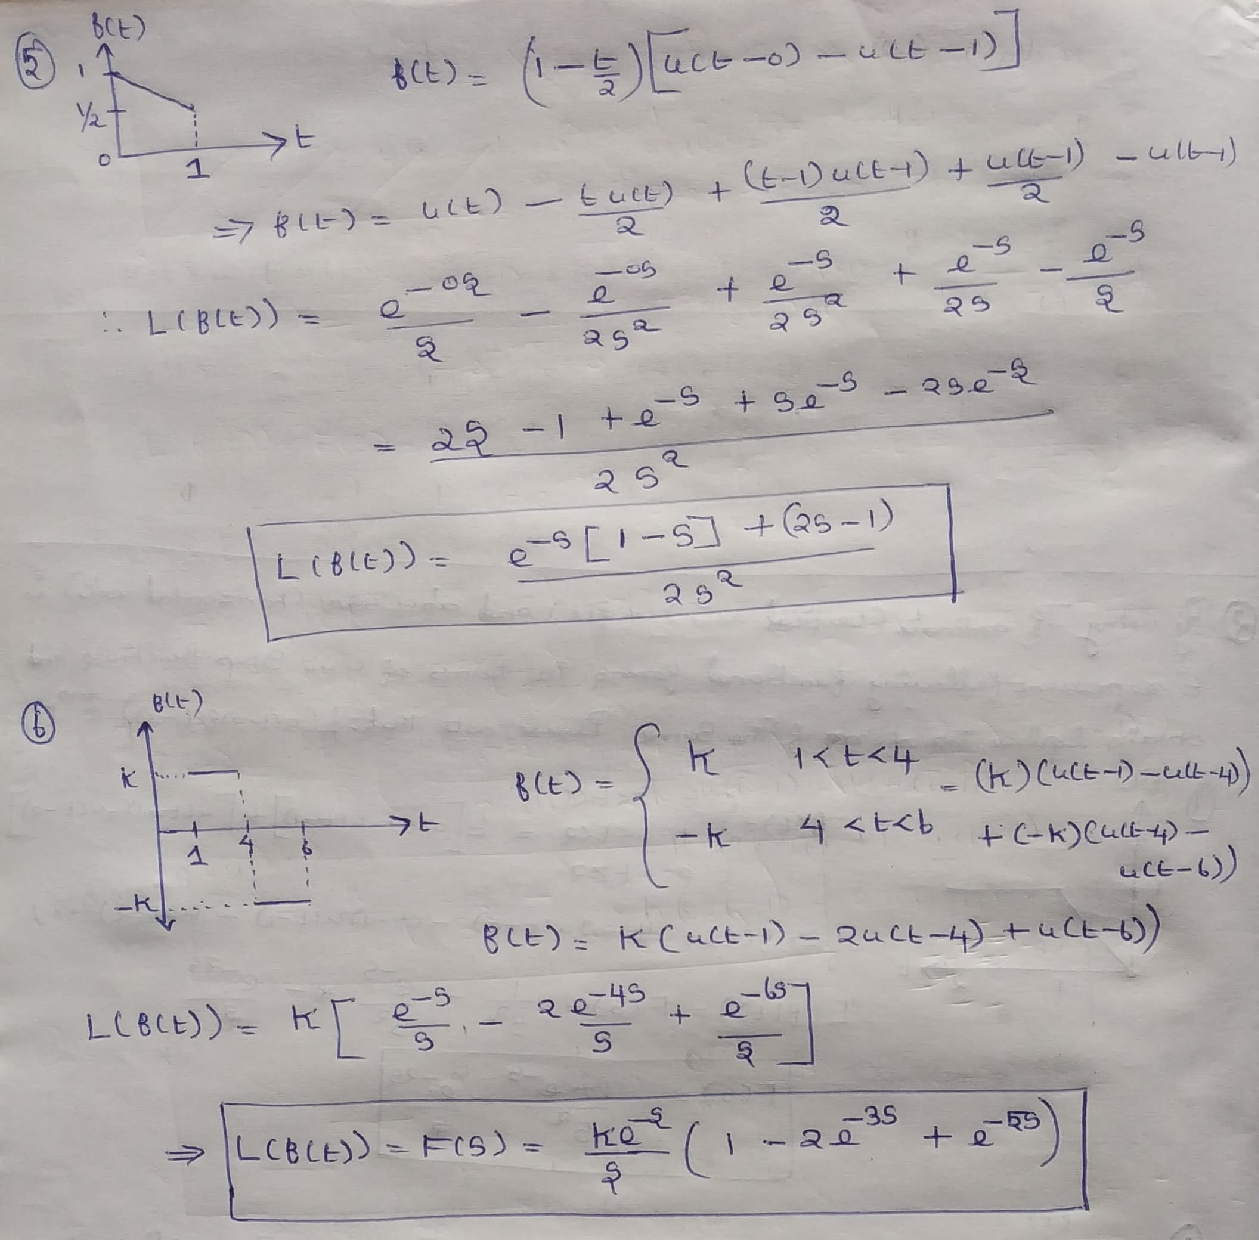
\includepdf[pages=-,pagecommand={},width=\textwidth]{CF_Assignment02.pdf}
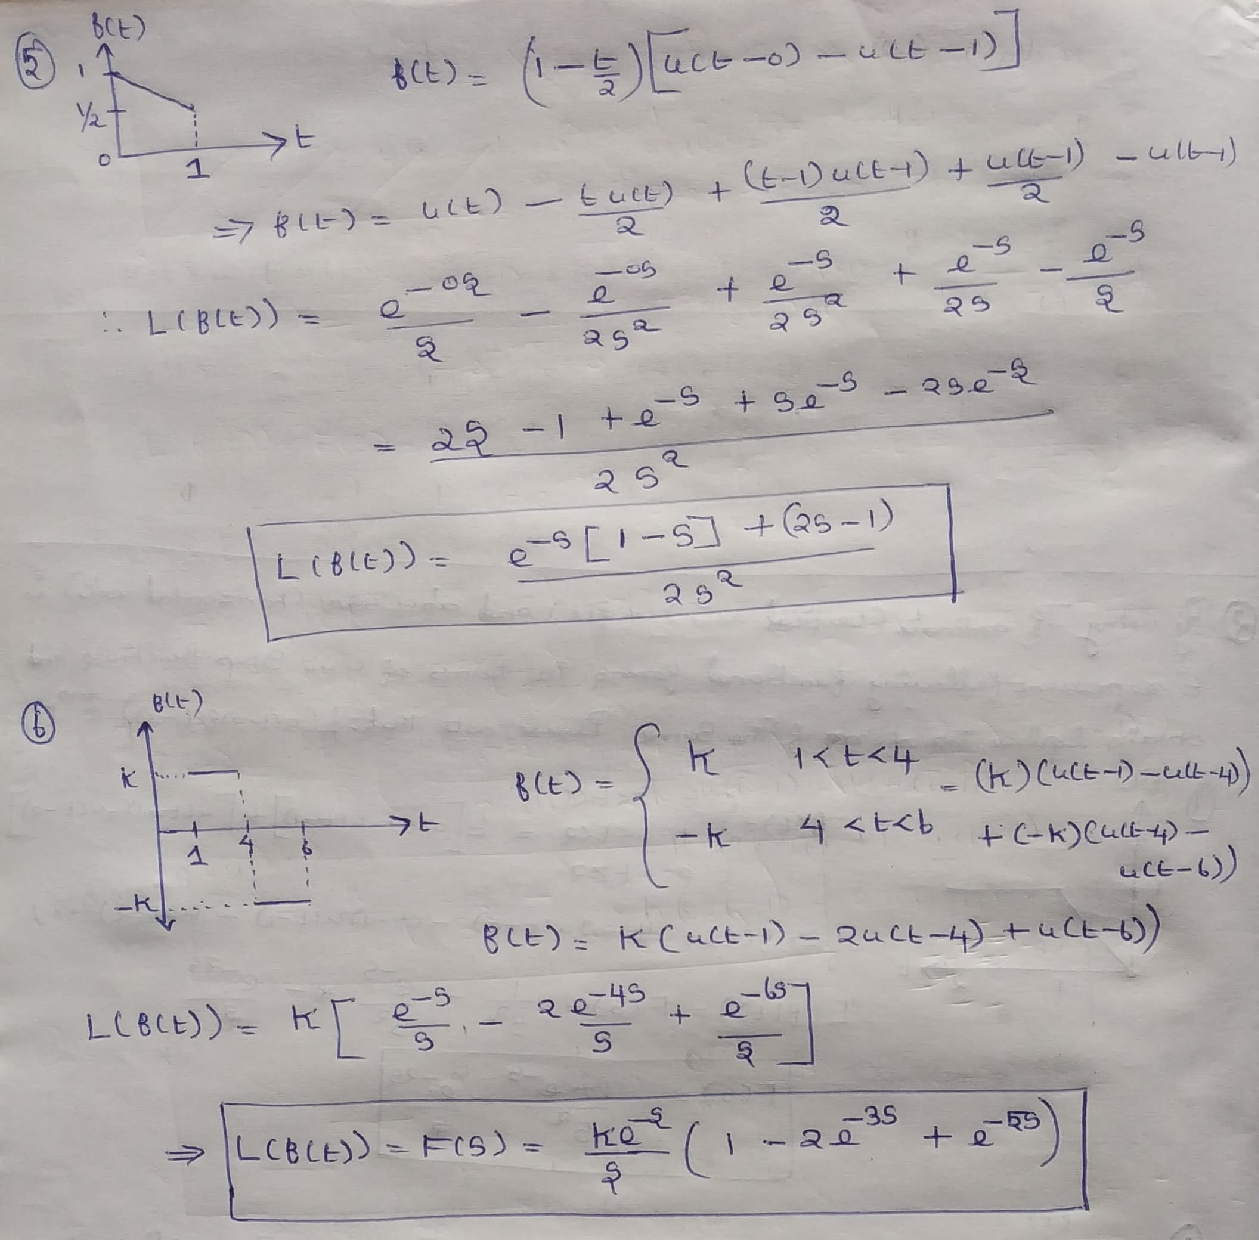
\includepdf[pages=-,pagecommand={},landscape=true,fitpaper=true]{CF_Assignment02.pdf}
%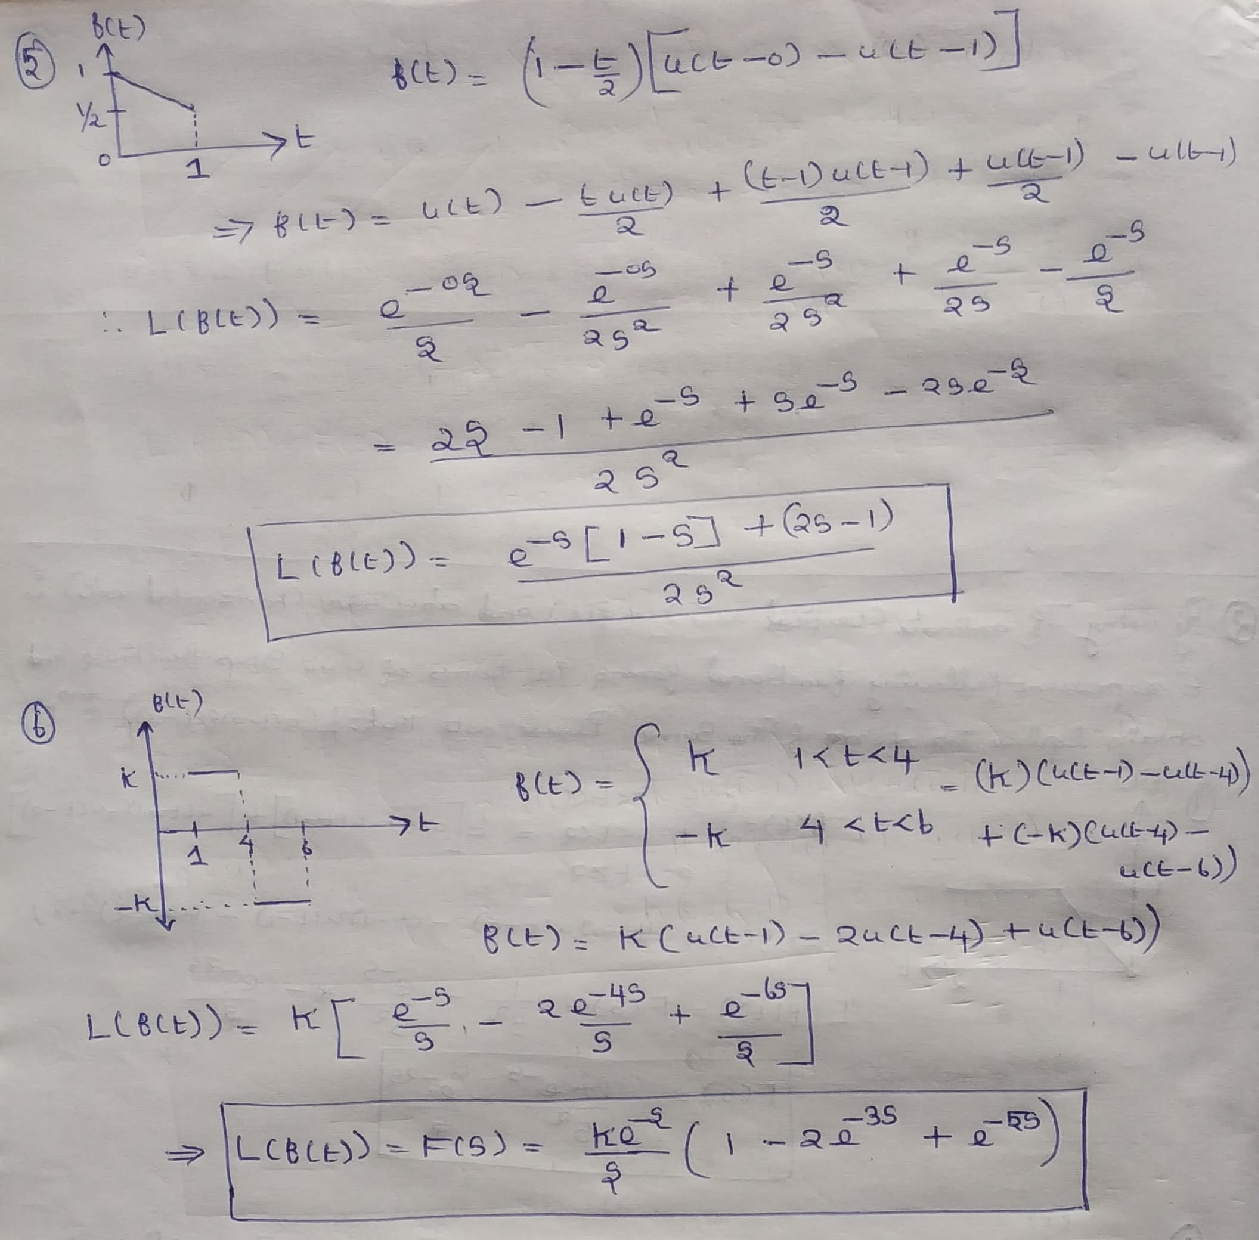
\includepdf[frame=true,pages=-,fitpaper=true,width=\textwidth]{CF_Assignment02.pdf}
\end{document}
